% !TeX root = pres.tex

\documentclass{beamer}

\usetheme{CambridgeUS}
\usecolortheme{whale}
\usefonttheme{professionalfonts}

\title[Master thesis]{Practical implementation of a parametrized binary matrix clustering algorithm}

\author[Leirvåg, Oskar]
{
    \textit{Student:} Oskar Leirvåg
    \and
    \textit{Mentor:} Petr A. Golovach
}

\institute[UiB] {
  Institute of Informatics: Algorithms \\
  University of Bergen
}

\date[\today]{\today}
%Bookmarks
\usepackage[colorlinks=true,urlcolor=cyan,linkcolor=black,citecolor=red,bookmarksopen=true]{hyperref}
\usepackage{bookmark}

\usepackage[utf8]{inputenc}
\usepackage{amsmath}
\usepackage{amsthm}
\usepackage[framemethod=TikZ]{mdframed}
\usepackage{pgf,tikz}
\usepackage{mathrsfs}
\usepackage{listings}
\usepackage{amssymb}
\usepackage{url}
\usepackage{hyperref}
\usepackage{graphicx}

% Ensure that by default, figures have no caption
\usepackage{caption}
\DeclareCaptionFormat{nocaption}{}
\captionsetup{format=nocaption,aboveskip=0pt,belowskip=0pt}

\usepackage[Export]{adjustbox} % Used to constrain images to a maximum size
\adjustboxset{max size={0.9\linewidth}{0.9\paperheight}}

\usepackage{float}
\floatplacement{figure}{H} % forces figures to be placed at the correct location

\usepackage{enumerate} % Needed for markdown enumerations to work

\usepackage[mathletters]{ucs}

\usepackage{titling} %Remove insane whitespaces

%Margins
\usepackage{geometry}
\geometry{a4paper, margin=3cm}

%Algorithms
\usepackage{algorithm, algorithmicx}
\usepackage{algpseudocode}
\newcommand{\myFigure}[3]{\begin{figure}[h!]\centering\includegraphics[scale=#1]{figures/#2}\caption{#3}\end{figure}}

\newtheorem{theoremdefinition}{\textbf{Definition}}
\newtheorem{theoremlemma}{\textbf{Lemma}}

% Algorithmic ForEach
\algnewcommand\algorithmicforeach{\textbf{foreach}}
\algdef{S}[FOR]{ForEach}[1]{\algorithmicforeach\ #1\ \algorithmicdo}

%Algorithmic ForTo
\algdef{S}[FOR]{ForTo}[2]{\algorithmicfor\ #1 \textbf{to} #2\ \algorithmicdo}

%Algorithmic Input
\algnewcommand\algorithmicinput{\textbf{Input:}}
\algnewcommand\Input{\item[\algorithmicinput]}

%Algorithmic Output
\algnewcommand\algorithmicoutput{\textbf{Output:}}
\algnewcommand\Output{\item[\algorithmicoutput]}

%FancyRef
%\newcommand*{\fancyrefthmlabelprefix}{thm}
\newcommand*{\mref}[1]{\hyperref[#1]{\fref{#1}}}
\newcommand*{\Mref}[1]{\hyperref[#1]{\Fref{#1}}}

\newcommand*{\fancyrefalglabelprefix}{alg}
\frefformat{vario}{\fancyrefalglabelprefix}{algorithm\fancyrefdefaultspacing#1}
\Frefformat{vario}{\fancyrefalglabelprefix}{Algorithm\fancyrefdefaultspacing#1}

\newcommand*{\fancyrefproblabelprefix}{prob}
\frefformat{vario}{\fancyrefproblabelprefix}{problem\fancyrefdefaultspacing#1}
\Frefformat{vario}{\fancyrefproblabelprefix}{Problem\fancyrefdefaultspacing#1}

\newcommand*{\fancyreflemlabelprefix}{lem}
\frefformat{vario}{\fancyreflemlabelprefix}{lemma\fancyrefdefaultspacing#1}
\Frefformat{vario}{\fancyreflemlabelprefix}{Lemma\fancyrefdefaultspacing#1}

\newcommand*{\fancyrefdeflabelprefix}{def}
\frefformat{vario}{\fancyrefdeflabelprefix}{definition\fancyrefdefaultspacing#1}
\Frefformat{vario}{\fancyrefdeflabelprefix}{Definition\fancyrefdefaultspacing#1}

\newenvironment{problem}[1][]{
    \mdfsetup{
        frametitle={
                \tikz[baseline=(current bounding box.east),outer sep=0pt]
                \node[anchor=east,rectangle,fill=white!20]
                {\strut ~#1};}
    }

    \mdfsetup{
        innertopmargin=10pt,linecolor=black!30,
        linewidth=1pt,topline=true,
        roundcorner=5pt,
        frametitleaboveskip=\dimexpr-\ht\strutbox\relax
    }

    \begin{mdframed}[]\relax}{
    \end{mdframed}}

\begin{document}

\frame{\titlepage}

\section{Introduction}
\subsection{Clustering}

\begin{frame}
  \begin{block}{Clustering}
    Collecting objects into groups by, \textit{s.t.} each object is \textit{closer}
    to the objects in the same group, than those in other groups, by some measure.
  \end{block}

  In itself, it is mainly a concept, and there exist several different types. Still
  it is the main task in several forms of statistical data-analysis, data mining and
  maybe most commonly known machine-learning.

  Here we will be talking about a specific \alert{centroid-based clustering} algorithm.
\end{frame}

\begin{frame}
  \begin{block}{Centroid-based clustering}
    A form of clustering where we produce or select a single object, not necessarily
    from the original data-set, to represent each cluster.
  \end{block}

  In other terms, instead of producing these groups \textit{(e.g. clusters)}, we will
  from these groups find a \textit{center} or \textit{average}. Thus maybe even
  ignoring the original data from that point on.
\end{frame}

\begin{frame}
  \begin{figure}
    \centering
    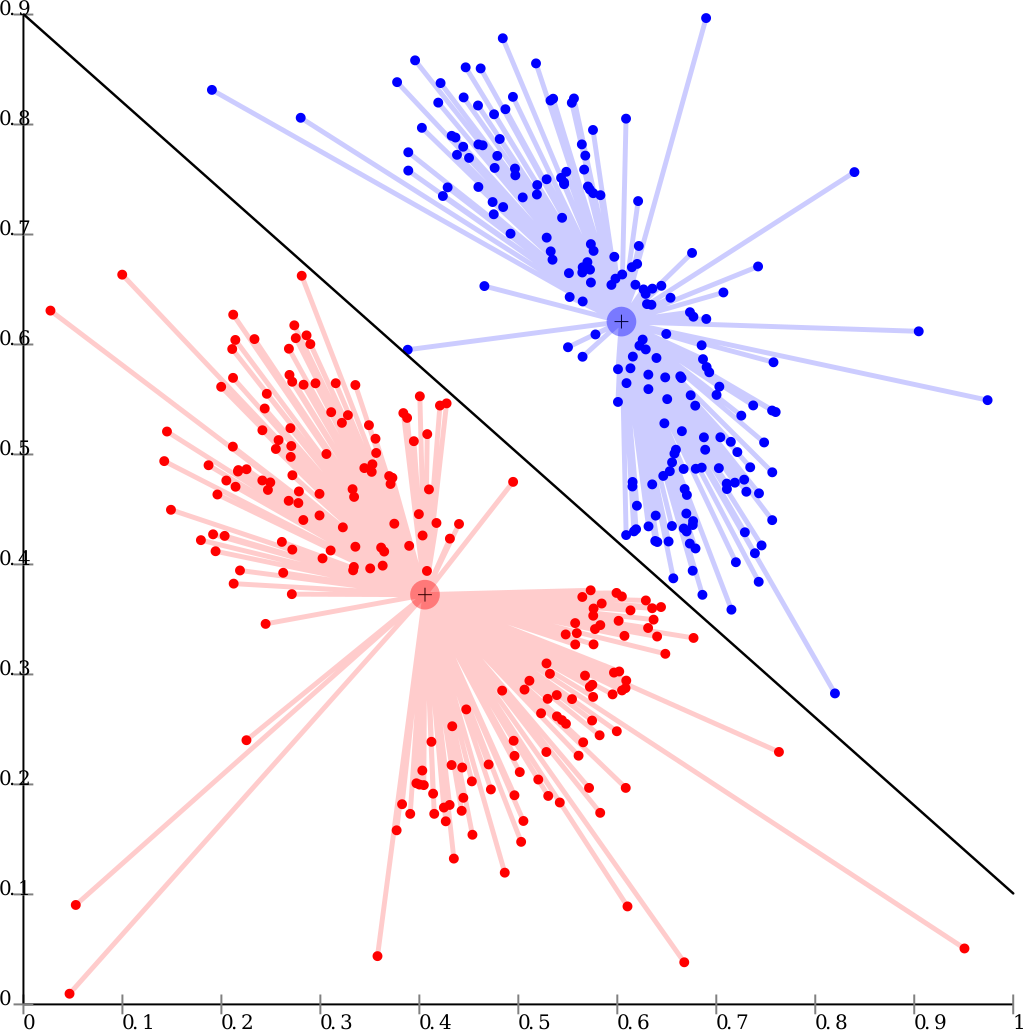
\includegraphics[height=0.75\textheight]{figures/1024px-KMeans-density-data.svg.png}
    \caption{from \cite{cluster:picture}}
  \end{figure}
\end{frame}

\subsection{Binary data}
\begin{frame}
  The data we will be using is \alert{binary vectors}, which will be
  clustered by their \alert{Hamming distance}, noted by $d_H(x,y)$.

  \begin{block}{Hamming distance}
    The Hamming distance between two binary vectors $x,y \in \{0,1\}^m$
    where $x=(x_1,...,x_m)^T$ and $y=(y_1,...,y_m)^T$, is
    \[
      d_H(x,y)= \sum_{i = 1}^{m} |x_i - y_i|
    \]
  \end{block}
\end{frame}

\begin{frame}
  \begin{block}{Example}
    Given a streaming services data on whether any user likes a given movie,
    we might want to create a recommendation service for new users.
    If we can classify our users into groups that share mostly the same taste in movies, then
    the "average-user" or centres of the classifications would be a "super user" most likely to share the same movie
    interest with any other user in the same classification.
  \end{block}
\end{frame}

\begin{frame}
  From the example, it may be clear that the vectors can represent a
  \alert{binary matrix}, in a clearer way. Thus further we will use columns of binary
  matrices, as the main objects.

  \begin{block}{Binary matrix}
    \[
      A_{m,n} =
      \begin{pmatrix}
        a_{1,1} & a_{1,2} & \cdots & a_{1,n} \\
        a_{2,1} & a_{2,2} & \cdots & a_{2,n} \\
        \vdots  & \vdots  & \ddots & \vdots  \\
        a_{m,1} & a_{m,2} & \cdots & a_{m,n}
      \end{pmatrix}
    \]
  \end{block}
\end{frame}

\subsection{Example}

\begin{frame}
  \begin{block}{$8 \times 8$matrix example}
    \[
      \begin{matrix}
        1 & 0 & 1 & 0 & 1 & 1 & 1 & 1 \\
        0 & 1 & 0 & 1 & 1 & 1 & 1 & 0 \\
        1 & 0 & 1 & 0 & 1 & 1 & 1 & 1 \\
        1 & 1 & 1 & 1 & 1 & 1 & 1 & 1 \\
        0 & 1 & 0 & 1 & 0 & 0 & 1 & 1 \\
        1 & 0 & 0 & 0 & 1 & 1 & 1 & 1 \\
        0 & 1 & 0 & 0 & 0 & 1 & 1 & 1 \\
        0 & 0 & 0 & 0 & 0 & 0 & 0 & 0
      \end{matrix} \quad \rightarrow \pause \quad \begin{matrix}
        1 & 1 \\
        0 & 1 \\
        1 & 1 \\
        1 & 1 \\
        0 & 1 \\
        0 & 1 \\
        0 & 1 \\
        0 & 0
      \end{matrix}
    \]
  \end{block}
\end{frame}

\section{Problem statement}

\subsection{Formal definition}
\begin{frame}
  \begin{block}{Binary r-Means}
    \begin{tabular}{p{0.1\textwidth}p{0.8\textwidth}}
      \textit{Input}: & An $n \times m$ binary matrix \textbf{A} with columns
      ($\textbf{a}^1,...,\textbf{a}^n$), a positive integer $\textbf{r}$ and a nonnegative
      integer $\textbf{k}$                                                                     \\

      \pause

      \textit{Task}:  & Decide whether there is a positive integer $\textbf{r}\sp{\prime} \leq
        \textbf{r}$, a partition $\{I_1, ..., I_{r\sp{\prime}}\}$ of indices $\{1,...,n\}$ and vectors
      $(\textbf{c}^1,...,\textbf{c}^{r\sp{\prime}}) \in \{0,1\}^m$ such that

      \[
        \sum_{i = 1}^{r\sp{\prime}} \sum_{j \in I_i} d_H(c^i, a^j) \leq k
      \]
    \end{tabular}
  \end{block}
\end{frame}

\subsection{Task and motivation}
\begin{frame}
  \begin{block}{Motivation}
    Not many algorithms for clustering binary vectors exactly. And due to the
    nature of the existing algorithms, their practical implementation should be tested
  \end{block}

  \begin{block}{Task}
    \begin{enumerate}
      \item Implement a practical version of the \alert{Binary r-Means} algorithm from
            \cite{fomin_golovach_panolan_2020}
      \item Generate and run test-cases automatically with different parameters on
            the implementation
      \item Analyse the actual runtime till completion
    \end{enumerate}
  \end{block}
\end{frame}

\section{The algorithm}
\begin{frame}
  The algorithm can be explained in three parts
  \begin{enumerate}
    \item<1-> The pre-processing part \textit{(e.g. the kernel)}
    \item<2-> The recursive branching clustering part
    \item<3-> The dynamic reconstruction part
  \end{enumerate}
\end{frame}

\subsection{Kernel}
\begin{frame}
  As the first part is to act as a kernel, there are many requirements. All that is
  explained by the following

  \pause

  \begin{theoremlemma}{\cite[Lemma 5]{fomin_golovach_panolan_2020}}
    Given an instance $(A,r,k)$ of Binary r-Means, Algorithm 1 runs in $O(n^2m)$ time
    and either correctly concludes that $(A,r,k)$ is a no-instance of Binary r-Means and
    returns NO or returns $s \leq r$ matrices $A_1, \dots, A_s$ such that

    \begin{itemize}
      \item<3-> $(A,r,k)$ is a yes-instance of Binary r-Means if and only if there are positive
      $r_1,\dots,r_s$ and nonnegative $k_1,\dots,k_s$ such that $(i)$ $r_1 + \dots + r_s \leq r$,
      $(ii)$ $k_1 + \dots + k_s \leq k$, and $(iii)$ $(A_i,r_i,k_i)$ is a yes-instance of Binary
      r-Means for every $i\in\{1,\dots,s\}$
      \item<4-> for every $i\in\{1,\dots,s\}$, $A_i$ is $m_i \times n_i$ matrix with
      $m_i \leq max\{(\ell_i - 1)k, 1\}$, where $\ell_i$ is the number of distinct columns
      of $A_i$ and $n_1 + \dots + n_s \leq (k+1)(k+r)$
      \item<5-> the total number of distinct columns in $A_1,\dots,A_s$ is at most $k+r$
    \end{itemize}
  \end{theoremlemma}
\end{frame}

\begin{frame}
  To achieve that, lets first look at the direct wanted functionality and define it as follows

  \begin{block}{Pre-processing}
    \begin{tabular}{r l}
      \textit{Input:}  & An $n \times m$ binary matrix $A=(a^1,...,a^n)$, $r > 0$, and $k \geq 0$ \\
      \textit{Output:} & A set $L$ of sub-matrices $A_1,\dots,A_s$
    \end{tabular}
  \end{block}

  \pause

  \begin{block}{Process}
    \begin{enumerate}
      \item<3-> Partition columns of $A$ into clusters of equal columns $I = {I_1, \dots, I_t}$ (\alert{initial clusters})
      and test if $t \ge k+r$
      \item<4-> Reduce any initial cluster of size $|I| \geq k+2$
      \item<5-> Greedily group the columns of the initial clusters, with columns of $d_H(I_a,I_b) \leq k$, call this new
      partition $L$
      \item<6-> Each set in the partition $L$ is now it's own matrix
      \item<7-> Remove \alert{Uniform rows}
    \end{enumerate}
  \end{block}
\end{frame}

\subsection{Clustering}
\begin{frame}
  \begin{block}{Binary r-Means}
    \begin{tabular}{r l}
      \textit{Input:}  & A set of indices $I \subseteq \{1,\dots,n\}$, a set of vectors
      $S \subseteq \{0,1\}^m$,                                                          \\
                       & and a nonnegative integer $d$                                  \\
      \textit{Output:} & A set of centres $S$
    \end{tabular}
  \end{block}


\end{frame}

\subsection{Reconstruction}
\begin{frame}
  \begin{block}{Reconstruction table $T[i,k^\prime]$}
    \begin{tabular}{lcl}
      $T[1, k^\prime]$ & $=$ & $f_1(k^\prime)$                                              \\
      $T[i, k^\prime]$ & $=$ & $min\{ min\{ T[ i-1, k_1 ] + f_i(k_2)$                       \\
                       &     & $|~ k_1 + k_2 = k^\prime, ~k_1 \wedge k_2 \geq 0\}, ~r+1 \}$
    \end{tabular}
  \end{block}
\end{frame}

\section{Testing}
\begin{frame}
  The initial goal of testing was to measure the actual runtime of the algorithm on different instances,
  so an automation was needed.

  \begin{block}{Testing algorithm}
    \begin{enumerate}
      \item<1-> Generate random binary matrix with solution within parameters
      \item<2-> Run algorithm on said matrix
      \item<3-> Upload runtime to database
    \end{enumerate}
  \end{block}
\end{frame}

\subsection{Variables}
\begin{frame}
  In testing, the random-generation algorithm would need to create not completely random inputs, but
  inputs which could be solved within or almost within; the parameters of $k$ and $r$. Thus we define
  the testing parameters

  \begin{block}{Variables}
    \begin{tabular}{lll}
      $h$ & $\rightarrow$ & \textit{\#initial clusters} used to generate              \\
      $d$ & $\rightarrow$ & \textit{\#random-bit-flips} performed on matrix           \\
      $r$ & $\rightarrow$ & the initial parameter $r$ that was given to the algorithm \\
      $k$ & $\rightarrow$ & the initial parameter $k$ that was given to the algorithm \\
    \end{tabular}
  \end{block}
\end{frame}

\subsection{Generating test cases}
\begin{frame}
  \begin{block}{Generate random binary matrix}
    \begin{enumerate}
      \item<1-> Generate \alert{h} random vectors
      \item<2-> While $|S| \leq n$ copy random vector from \alert{h} into $S$
      \item<3-> Flip a random bit $A[S]_{x,y}$, \alert{d} times
    \end{enumerate}
  \end{block}
\end{frame}

\section{Results}
\begin{frame}
  \begin{figure}
    \centering
    \includegraphics[height=0.75\textheight, page=4]{figures/Binary_matrix_runtime.pdf}
    \caption{Plot showing the average runtime of the algorithm in milliseconds \textit{(logarithmically)}
      over the parameter $k$, using matrices generates of size Width: $1000$ and Height:$1000$.}
  \end{figure}
\end{frame}

\begin{frame}
  \begin{figure}
    \centering
    \includegraphics[height=0.75\textheight, page=6]{figures/Binary_matrix_runtime.pdf}
    \caption{Plot showing the average runtime of the algorithm in milliseconds \textit{(logarithmically)}
      over the parameter $d$, using matrices generates of size Width: $1000$ and Height:$1000$.}
  \end{figure}
\end{frame}

\begin{frame}
  \begin{figure}
    \centering
    \includegraphics[height=0.75\textheight, page=3]{figures/Binary_matrix_runtime.pdf}
    \caption{Plot showing the average runtime of the algorithm in milliseconds \textit{(logarithmically)}
      over the parameter $k$, using matrices generates of size Width: $200$ and Height:$200$.}
  \end{figure}
\end{frame}

\begin{frame}
  \begin{figure}
    \centering
    \includegraphics[height=0.75\textheight, page=7]{figures/Binary_matrix_runtime.pdf}
    \caption{Plot showing the average runtime of the algorithm in milliseconds \textit{(logarithmically)}
      over the parameter $k$, all data from all test-runs with all matrices from this report, grouped by
      the size of the matrices.}
  \end{figure}
\end{frame}

\begin{frame}
  \begin{figure}
    \centering
    \includegraphics[height=0.75\textheight, page=2]{figures/Binary_matrix_runtime.pdf}
    \caption{Plot showing the average runtime of the algorithm in milliseconds \textit{(logarithmically)}
      over the parameter $k$, using matrices generates of size Width: $100$ and Height:$20$.}
  \end{figure}
\end{frame}

\begin{frame}
  \begin{figure}
    \centering
    \includegraphics[height=0.75\textheight, page=5]{figures/Binary_matrix_runtime.pdf}
    \caption{Plot showing the average runtime of the algorithm in milliseconds \textit{(logarithmically)}
      over the parameter $d$, using matrices generates of size Width: $100$ and Height:$20$.}
  \end{figure}
\end{frame}

\begin{frame}
  \begin{figure}
    \centering
    \includegraphics[height=0.75\textheight, page=1]{figures/Binary_matrix_runtime.pdf}
    \caption{Plot showing the average runtime of the algorithm in milliseconds \textit{(logarithmically)}
      over the parameter $k$, using all data from all test-runs with all matrices from this report.}
  \end{figure}
\end{frame}

\begin{frame}
  \begin{figure}
    \centering
    \includegraphics[height=0.75\textheight, page=8]{figures/Binary_matrix_runtime.pdf}
    \caption{Plot showing the average runtime of the algorithm in milliseconds \textit{(logarithmically)}
      over the parameter $d$, using all data from all test-runs with all matrices from this report, grouped by
      the size of the matrices.}
  \end{figure}
\end{frame}

\section{Presentation references}
\bibliography{extras/citation-db}
\bibliographystyle{apalike} %unsrt

\end{document}